% Options for packages loaded elsewhere
\PassOptionsToPackage{unicode}{hyperref}
\PassOptionsToPackage{hyphens}{url}
%
\documentclass[
  english,
  man,floatsintext]{apa6}
\usepackage{amsmath,amssymb}
\usepackage{lmodern}
\usepackage{ifxetex,ifluatex}
\ifnum 0\ifxetex 1\fi\ifluatex 1\fi=0 % if pdftex
  \usepackage[T1]{fontenc}
  \usepackage[utf8]{inputenc}
  \usepackage{textcomp} % provide euro and other symbols
\else % if luatex or xetex
  \usepackage{unicode-math}
  \defaultfontfeatures{Scale=MatchLowercase}
  \defaultfontfeatures[\rmfamily]{Ligatures=TeX,Scale=1}
\fi
% Use upquote if available, for straight quotes in verbatim environments
\IfFileExists{upquote.sty}{\usepackage{upquote}}{}
\IfFileExists{microtype.sty}{% use microtype if available
  \usepackage[]{microtype}
  \UseMicrotypeSet[protrusion]{basicmath} % disable protrusion for tt fonts
}{}
\makeatletter
\@ifundefined{KOMAClassName}{% if non-KOMA class
  \IfFileExists{parskip.sty}{%
    \usepackage{parskip}
  }{% else
    \setlength{\parindent}{0pt}
    \setlength{\parskip}{6pt plus 2pt minus 1pt}}
}{% if KOMA class
  \KOMAoptions{parskip=half}}
\makeatother
\usepackage{xcolor}
\IfFileExists{xurl.sty}{\usepackage{xurl}}{} % add URL line breaks if available
\IfFileExists{bookmark.sty}{\usepackage{bookmark}}{\usepackage{hyperref}}
\hypersetup{
  pdftitle={Choosing a car to optimize miles per gallon},
  pdfauthor={Marisa Casillas1},
  pdflang={en-EN},
  pdfkeywords={Fuel efficiency, transmission, engine size},
  hidelinks,
  pdfcreator={LaTeX via pandoc}}
\urlstyle{same} % disable monospaced font for URLs
\usepackage{graphicx}
\makeatletter
\def\maxwidth{\ifdim\Gin@nat@width>\linewidth\linewidth\else\Gin@nat@width\fi}
\def\maxheight{\ifdim\Gin@nat@height>\textheight\textheight\else\Gin@nat@height\fi}
\makeatother
% Scale images if necessary, so that they will not overflow the page
% margins by default, and it is still possible to overwrite the defaults
% using explicit options in \includegraphics[width, height, ...]{}
\setkeys{Gin}{width=\maxwidth,height=\maxheight,keepaspectratio}
% Set default figure placement to htbp
\makeatletter
\def\fps@figure{htbp}
\makeatother
\setlength{\emergencystretch}{3em} % prevent overfull lines
\providecommand{\tightlist}{%
  \setlength{\itemsep}{0pt}\setlength{\parskip}{0pt}}
\setcounter{secnumdepth}{-\maxdimen} % remove section numbering
% Make \paragraph and \subparagraph free-standing
\ifx\paragraph\undefined\else
  \let\oldparagraph\paragraph
  \renewcommand{\paragraph}[1]{\oldparagraph{#1}\mbox{}}
\fi
\ifx\subparagraph\undefined\else
  \let\oldsubparagraph\subparagraph
  \renewcommand{\subparagraph}[1]{\oldsubparagraph{#1}\mbox{}}
\fi
% Manuscript styling
\usepackage{upgreek}
\captionsetup{font=singlespacing,justification=justified}

% Table formatting
\usepackage{longtable}
\usepackage{lscape}
% \usepackage[counterclockwise]{rotating}   % Landscape page setup for large tables
\usepackage{multirow}		% Table styling
\usepackage{tabularx}		% Control Column width
\usepackage[flushleft]{threeparttable}	% Allows for three part tables with a specified notes section
\usepackage{threeparttablex}            % Lets threeparttable work with longtable

% Create new environments so endfloat can handle them
% \newenvironment{ltable}
%   {\begin{landscape}\centering\begin{threeparttable}}
%   {\end{threeparttable}\end{landscape}}
\newenvironment{lltable}{\begin{landscape}\centering\begin{ThreePartTable}}{\end{ThreePartTable}\end{landscape}}

% Enables adjusting longtable caption width to table width
% Solution found at http://golatex.de/longtable-mit-caption-so-breit-wie-die-tabelle-t15767.html
\makeatletter
\newcommand\LastLTentrywidth{1em}
\newlength\longtablewidth
\setlength{\longtablewidth}{1in}
\newcommand{\getlongtablewidth}{\begingroup \ifcsname LT@\roman{LT@tables}\endcsname \global\longtablewidth=0pt \renewcommand{\LT@entry}[2]{\global\advance\longtablewidth by ##2\relax\gdef\LastLTentrywidth{##2}}\@nameuse{LT@\roman{LT@tables}} \fi \endgroup}

% \setlength{\parindent}{0.5in}
% \setlength{\parskip}{0pt plus 0pt minus 0pt}

% \usepackage{etoolbox}
\makeatletter
\patchcmd{\HyOrg@maketitle}
  {\section{\normalfont\normalsize\abstractname}}
  {\section*{\normalfont\normalsize\abstractname}}
  {}{\typeout{Failed to patch abstract.}}
\patchcmd{\HyOrg@maketitle}
  {\section{\protect\normalfont{\@title}}}
  {\section*{\protect\normalfont{\@title}}}
  {}{\typeout{Failed to patch title.}}
\makeatother
\shorttitle{Optimizing miles per gallon}
\keywords{Fuel efficiency, transmission, engine size}
\usepackage{csquotes}
\ifxetex
  % Load polyglossia as late as possible: uses bidi with RTL langages (e.g. Hebrew, Arabic)
  \usepackage{polyglossia}
  \setmainlanguage[]{english}
\else
  \usepackage[main=english]{babel}
% get rid of language-specific shorthands (see #6817):
\let\LanguageShortHands\languageshorthands
\def\languageshorthands#1{}
\fi
\ifluatex
  \usepackage{selnolig}  % disable illegal ligatures
\fi
\newlength{\cslhangindent}
\setlength{\cslhangindent}{1.5em}
\newlength{\csllabelwidth}
\setlength{\csllabelwidth}{3em}
\newenvironment{CSLReferences}[2] % #1 hanging-ident, #2 entry spacing
 {% don't indent paragraphs
  \setlength{\parindent}{0pt}
  % turn on hanging indent if param 1 is 1
  \ifodd #1 \everypar{\setlength{\hangindent}{\cslhangindent}}\ignorespaces\fi
  % set entry spacing
  \ifnum #2 > 0
  \setlength{\parskip}{#2\baselineskip}
  \fi
 }%
 {}
\usepackage{calc}
\newcommand{\CSLBlock}[1]{#1\hfill\break}
\newcommand{\CSLLeftMargin}[1]{\parbox[t]{\csllabelwidth}{#1}}
\newcommand{\CSLRightInline}[1]{\parbox[t]{\linewidth - \csllabelwidth}{#1}\break}
\newcommand{\CSLIndent}[1]{\hspace{\cslhangindent}#1}

\title{Choosing a car to optimize miles per gallon}
\author{Marisa Casillas\textsuperscript{1}}
\date{}


\authornote{

Please email \href{mailto:mcasillas@uchicago.edu}{\nolinkurl{mcasillas@uchicago.edu}} for questions about this important research.

Correspondence concerning this article should be addressed to Marisa Casillas, Rosenwald Hall, UChicago. E-mail: \href{mailto:mcasillas@uchicago.edu}{\nolinkurl{mcasillas@uchicago.edu}}

}

\affiliation{\vspace{0.5cm}\textsuperscript{1} University of Chicago}

\abstract{
Gas is expensive and burning it is bad for environmental health. How do I choose a car to optimize my gas mileage? We examine a few potential variables to help answer this question.
}



\begin{document}
\maketitle

\hypertarget{introduction}{%
\section{Introduction}\label{introduction}}

In the \texttt{mtcars} dataset (Henderson \& Velleman, 1981) there are 32 cars documented, from 0 brands. The unique car types documented are: Mazda RX4, Mazda RX4 Wag, Datsun 710, Hornet 4 Drive, Hornet Sportabout, Valiant, Duster 360, Merc 240D, Merc 230, Merc 280, Merc 280C, Merc 450SE, Merc 450SL, Merc 450SLC, Cadillac Fleetwood, Lincoln Continental, Chrysler Imperial, Fiat 128, Honda Civic, Toyota Corolla, Toyota Corona, Dodge Challenger, AMC Javelin, Camaro Z28, Pontiac Firebird, Fiat X1-9, Porsche 914-2, Lotus Europa, Ford Pantera L, Ferrari Dino, Maserati Bora, and Volvo 142E. The mean mpg is 20.09 (median = 19.20; sd = 6.03; range = 10.40--33.90). The cars range in number of cylinders from 4 to 8, though there are no cars with odd numbers of cylinders.

\begin{table}

\caption{\label{tab:summary-tbl}Brands included, along with average number of cylinders and average weight among the number of models included for each brand.}
\centering
\begin{tabular}[t]{l|r|r|r}
\hline
brand & \# Cylinders & Weight & \# models\\
\hline
Datsun & 4.0 & 2.3 & 1\\
\hline
Fiat & 4.0 & 2.1 & 2\\
\hline
Honda & 4.0 & 1.6 & 1\\
\hline
Lotus & 4.0 & 1.5 & 1\\
\hline
Porsche & 4.0 & 2.1 & 1\\
\hline
Toyota & 4.0 & 2.1 & 2\\
\hline
Volvo & 4.0 & 2.8 & 1\\
\hline
Ferrari & 6.0 & 2.8 & 1\\
\hline
Mazda & 6.0 & 2.8 & 2\\
\hline
Valiant & 6.0 & 3.5 & 1\\
\hline
Merc & 6.3 & 3.5 & 7\\
\hline
Hornet & 7.0 & 3.3 & 2\\
\hline
AMC & 8.0 & 3.4 & 1\\
\hline
Cadillac & 8.0 & 5.2 & 1\\
\hline
Camaro & 8.0 & 3.8 & 1\\
\hline
Chrysler & 8.0 & 5.3 & 1\\
\hline
Dodge & 8.0 & 3.5 & 1\\
\hline
Duster & 8.0 & 3.6 & 1\\
\hline
Ford & 8.0 & 3.2 & 1\\
\hline
Lincoln & 8.0 & 5.4 & 1\\
\hline
Maserati & 8.0 & 3.6 & 1\\
\hline
Pontiac & 8.0 & 3.9 & 1\\
\hline
\end{tabular}
\end{table}

We show the unique brands along with their average number of cylinders, average weight, and number of models represented in the dataset in Table \ref{tab:summary-tbl}. We summarize our findings in subsection \ref{results} and note that subsection \ref{references-we-love} is unrelated to this report.

\hypertarget{results}{%
\section{Results}\label{results}}

We modeled mileage with a linear mixed-effects regression, including fixed effects of number of cylinders (numeric), transmission (automatic or manual), and their interaction, as well as a random effect of brand.\footnote{\texttt{lmer(mileage\ \textasciitilde{}\ cylinders\ *\ transmission\ +\ (1\textbar{}brand),\ data)}} Increases in number of cylinders was associated with significant decreases in mileage (\emph{B} = -1.59, \emph{SE} = 0.36, \emph{t} = -4.41). Meanwhile, manual transmissions were associated with significant increases in mileage compared to automatic ones (\emph{B} = 14.11, \emph{SE} = 3.94, \emph{t} = 3.59). That said, the decrease in mileage with more cylinders was significantly greater for manual transmission vehicles than automatic ones (\emph{B} = -1.73, \emph{SE} = 0.68, \emph{t} = -2.55).

\begin{figure}
\centering
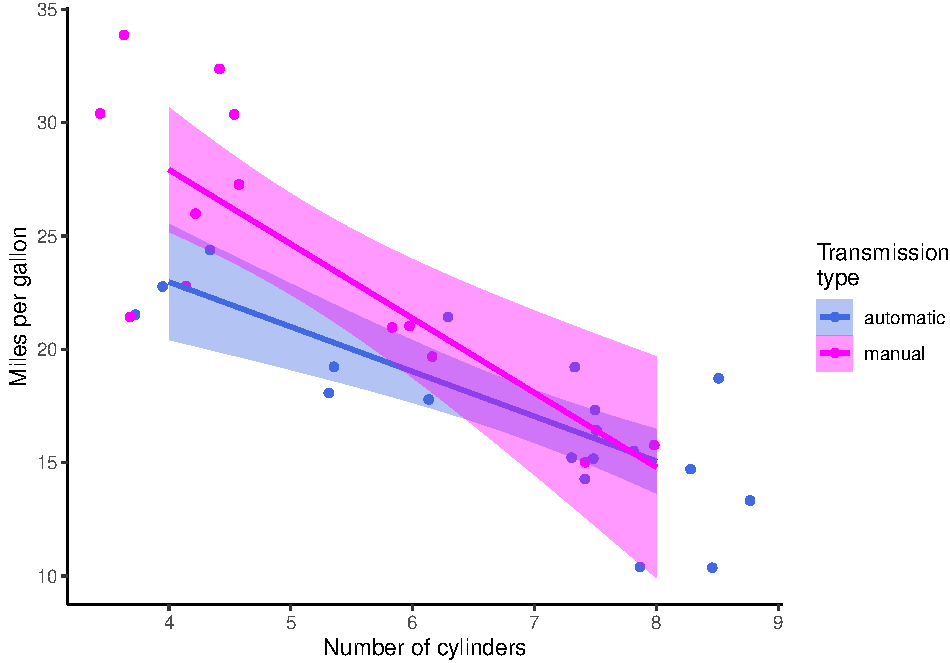
\includegraphics{mpg-report-papaja_files/figure-latex/plot-primary-results-1.pdf}
\caption{\label{fig:plot-primary-results}Miles per gallon as a function of nunber of cylinders and transmission type in the \texttt{mtcars} dataset.}
\end{figure}

These effects are visualized in Figure \ref{fig:plot-primary-results}.

\hypertarget{discussion}{%
\section{Discussion}\label{discussion}}

In this study we investigated the relationship between miles per gallon, number of cylinders, and transmission type in the \texttt{mtcars} dataset. Unsurprisingly, cars with more cylinders and cars with automatic transmissions had lower mileage. The effect of transmission depended on the number of cylinders, such that the mileage benefit associated with manual transmissions decreased for cars with more cylinders. Based on these data, someone trying to maximize their mileage should choose a manual transmission, low-cylinder vehicle.

\hypertarget{references-we-love}{%
\subsection{References we love}\label{references-we-love}}

You may want to cite references in different formats depending on the surrounding sentential context, e.g.: Casillas, in her (2022) course, states that Rmarkdown is awesome. Rmarkdown is awesome (Casillas, 2021a, 2022; Xie, Allaire, \& Grolemund, 2018). Rmarkdown is awesome (Casillas, 2022; e.g., Xie, Allaire, \& Grolemund, 2018). Same-year, same-author publications are automatically disambiguated (e.g., Casillas, 2021a, 2021b). We learned all about ggplot (see Wickham \& Grolemund, 2016, ch.~1). We learned about ggplot with Wickham and Grolemund (2016, ch.~1).

This reproducible manuscript is written in Rmarkdown (Xie, Allaire, \& Grolemund, 2018), using the lme4 (Bates, Mächler, Bolker, \& Walker, 2015) to run statistical models and ggplot2 (Wickham, 2016) within the tidyverse package (Wickham \& Grolemund, 2016) to generate plots.

\newpage

\hypertarget{references}{%
\section{References}\label{references}}

\begingroup
\setlength{\parindent}{-0.5in}
\setlength{\leftskip}{0.5in}

\hypertarget{refs}{}
\begin{CSLReferences}{1}{0}
\leavevmode\hypertarget{ref-lme4}{}%
Bates, D., Mächler, M., Bolker, B., \& Walker, S. (2015). Fitting linear mixed-effects models using {lme4}. \emph{Journal of Statistical Software}, \emph{67}(1), 1--48. \url{https://doi.org/10.18637/jss.v067.i01}

\leavevmode\hypertarget{ref-casillas2021r}{}%
Casillas, M. (2021a). {Reproducible science is great}. Various manuscripts.

\leavevmode\hypertarget{ref-casillas2021productive}{}%
Casillas, M. (2021b). {What a productive year}. Two publications!!

\leavevmode\hypertarget{ref-casillas2022d2mr}{}%
Casillas, M. (2022). {From Data to Manuscript in R}. UChicago coursework.

\leavevmode\hypertarget{ref-douglas2022introduction}{}%
Douglas, A., Roos, D., Mancini, F., Couto, A., \& Lusseau, D. (2022). {An Introduction to R}. https://intro2r.com/.

\leavevmode\hypertarget{ref-henderson1981building}{}%
Henderson, H. V., \& Velleman, P. F. (1981). Building multiple regression models interactively. \emph{Biometrics}, 391--411.

\leavevmode\hypertarget{ref-tierney2020rmarkdown}{}%
Tierney, N. J. (2020). {RMarkdown for Scientists}. https://rmd4sci.njtierney.com/.

\leavevmode\hypertarget{ref-ggplot2}{}%
Wickham, H. (2016). \emph{ggplot2: Elegant graphics for data analysis}. Springer-Verlag New York. Retrieved from \url{https://ggplot2.tidyverse.org}

\leavevmode\hypertarget{ref-wickham2016r4ds}{}%
Wickham, H., \& Grolemund, G. (2016). \emph{R for data science: Import, tidy, transform, visualize, and model data}. O'Reilly Media, Inc.

\leavevmode\hypertarget{ref-xie2018bookdown}{}%
Xie, Y., Allaire, J. J., \& Grolemund, G. (2018). \emph{R markdown: The definitive guide}. Chapman; Hall/CRC.

\end{CSLReferences}

\endgroup


\end{document}
